\chapter{Neoclassical Theories of Production and Growth} 
\label{chapter-growth}

\epigraph{It may be tempting to specify an aggregate production function that directly relates primary factors to final output, as is customary in much economic analysis. This standard simplification is often inadequate, however, because cities are characterized by increasing returns to scale and the way in which such increasing returns are generated has potentially important policy implications. In particular, detailed assumptions are needed about labor, the nature of products, the production function of individual firms, the input-output structure that links firms, and how firms compete.' \cite{spenceUrbanizationGrowth2009}}

The \gls{neoclassical} approaches to economic analysis built on the classical framework. They added  mathematical modelling and the use of calculus. Calculus made it much easier to derive formal statements of what came to be called ``marginal conditions', or rules for efficient choice. It also allowed economists to derive clear rules for complex cases that were very difficult to state verbally. For example, the utilitarian goal of `the greatest good for the greatest number' which is comprehensible but vague could be translated into a guideline expressed in terms of the sums of individual marginal utilities equalling the marginal social cost for each good. 

%*E THIS PARAGRAPH SEEMS TO MOVE VERY FAST %i THINK YOU NEED TO EXPLIAN MARGINAL CONDITIONS IN MORE DETAIL, REALLY MAKE THAT CLEAR THEN BUILD OUT THE UTILITARIAN GOAL AS MORE OF A FLESHED OUT EXAMPLE. IT SEEMS LIKE THE SKELETON OF WHAT YOU NEED TO INTRODUCE THESE CONCEPTS CLEARLY IS HERE BUT NOT ENOUGH. 

The results of this new style are analytically more precise than the verbal statements they replace, and more easily communicated accurately for those with some mathematical skill. The approach also tend to lay bare the precise condition - the background assumptions- that must hold for results to be true. A cost of this progress is that economics became less accessible for many people. 

It is important to remember that neoclassical economics did not overthrow the insights of the classical economists. It provided increased precision and power, and it shifted attention from questions of class and distribution to deriving efficiency conditions. Economics became less a collection of great thoughts about the economy and more a mathematical edifice that embodied most of those thoughts in a rigorously consistent way and was the path to ever more arcane insights.
*E WHILE THIS IS INTERESTING AS AN ACCOUNT OF THE RELATIONSHIP BETWEEN ECONOMICS AND THE PUBLIC, I'M NOT SURE HOW IT SETS UP WHERE YOU ARE GOING WITH THIS CHAPTER. CAN YOU BRING IT BACK TO RENT OR DISTRIBUTION, HOW THE NEW APPROACHES RELATE TO PROBLEMS YOU ARE LOOKING AT IN THIS THESIS?

\section{Neoclassical production theory}
The concept of a production function used by the increasingly mathematical neoclassical economists and  the rapidly developing statistical techniques  naturally led to attempts to identify the precise \gls{functional form} that would describe the contributions of labour, capital, and income to output.
*E COULD YOU FLESH THIS OUT, ADD EXAMPLES % ALSO MAYBE ADD WHAT WAS HAPPENING AT THE TIME, WHAT WERE THE PEOPLE LOOKING AT WHEN THEY STARTED TO APPLY THESE TOOLS TO THESE QUESTIONS. THIS MIGHT BE A GOOD PLACE TO REFERENCE BACK TO PREVIOUS PARTS ABOUT MARGINALISTS TO SET CONTEXT. 
 
\subsection{Classical rent theory using neoclassical notation}
Ricardo, for example, did not write down a formal production function as later \gls{neoclassical} theorists would\footnote{He did generate numerical examples to demonstrate comparative advantage, and others, such as the physiocrats, von Th\"unen and Marx developed models still cited today, but these were not central for classical theorizing. }, but his verbal production theory can be put in the notation neoclassical economists later developed. In modern notation, Ricardo's production model can be written: 
*THIS IS CONFUSING DID YOU PUT IT IN THIS FORM OR DID THE MARGINALISTS. NOTE.. %JUST ABOVE YOU SAY THE MARGINALISTS STARTED TO DO THIS. iS THIS AN EXAMPLE? OR YOU DOING WHAT THEY ALSO DID? cLARIFY. OR THIS CONFUSION MIGHT JUST GO AWAY WHEN YOU FILL OUT MORE EXAMPLES ABOVE

\begin{equation} 
Y=F(K,L,N).
\label{eqn-production-ricardo}
\end{equation} 

where  $Y$ is output, $K$ is capital invested, $L$ is labour and $N$  is the natural resource land.\footnote{This makes it a three-factor model of production.  In principle any number of factors can be included.}  
Ricardo does not specify a functional form, but, %like mathematical neoclassical economists, 
he does assume diminishing returns to all factors. 

The  rent, $\mathcal{R}$, that the landlord receives is the total market value of the potatoes produced minus the cost of the capital employed in improving the land and the wage bill for the labour employed: 

\begin{equation} 
\mathcal{R}= PQ-rk-wl
\label{eqn-rent-ricardo}
\end{equation} 
Equation~\ref{eqn-rent-ricardo} makes it clear that the rent is a residual or a \gls{surplus}. The land is not paid for its services. The value of the land is the \gls{present discounted value} of the surplus it generates for the owner, that is what it would be worth paying now, to capture the future rents from that land.

Ricardo's analysis of rents  can be expressed by focusing only on land:

\begin{equation} 
Y=F(L,N).
\label{eqn-production-ricardo-2}
\end{equation} 
while most modern neoclassical treatments of production simplify by omitting land and emphasizing capital:\begin{equation} 
Y=F(K,L).
\label{eqn-production}
\end{equation}  
This makes sense for a number of reasons. The economy has shifted from agriculture to industry and the focus of economic theory has shifted to manufacturing processes.

%Furthermore, according to the Ricardian theory, rent is a surplus above cost. It does not, therefore enter into price. Land is a fixed factor for society as a whole that is not consumed in  the process of production.  Neoclassical treatments of production focus price determination based on the cost of the last unit used, the marginal  unit of input, while rents are generated on all of the inframarginal units, those units used earlier, which are more productive. The marginal unit of land generates no rents. In neoclassical analysis, the rents disappeared from view for this reason. This difference is at the heart of the distinction between classical and neoclassical economic theory. 
% #E this distinction is because of the actual structural difference in the societies? Also because of the differ tools? and apporaches? 

 %The Principles tells us that as cultivation is extended and exchange increases, profits fall while rents increase. 

Leaving land out, however, creates a problem in  the neoclassical growth theories we will examine below. John B. Davis \cite{davisRicardoTheoryProfit1993} noted that ``Questions arise, however, when one turns to exchange between a sector paying rent and one not.'' 
Under the assumption of perfectly competitive goods and factors markets as well as marginal productivity pricing of capital and labour, neoclassical growth requires technical change to be generated outside the model because there are no resources left to innovate if both factors of production are paid their marginal product.\footnote{This follows from Euler’s theorem: if, for a given level of technology $\bar A$ output Y is produced according to a \textbf{constant returns to scale} and twice continuously differentiable function of capital and labour $F(K, L, \bar A)$, Euler’s theorem implies that $F_K K + F_L L=Y$, where $F_i$ is the marginal product of factor $i$. Payments to  capital and labour take up the entire national product and no resources are left to finance the production of technology-improving innovations. are paid their marginal product.} 
If, however, land is reintroduced, as it must be in an urban model, there must be rents and there is therefore a surplus available for innovation.
\footnote{An alternative and common approach is to assume imperfect competition, which may be based on increasing returns to scale, in which case firms with market power may achieve a surplus. ``Although seldom modeled outside the monopolistic competition framework, market incompleteness and imperfect competition are central to the new growth theories'' (Gilles Duranton, Growth and imperfect competition on factor markets: Increasing returns and distribution, European Economic Review, 44-2, 2000, 255-280), Similarly, Sjak Smulders and Theo van de Klundert conclude that ``Growth is higher in a more concentrated market provided that market power of firms is not too high,'' (Imperfect competition, concentration and growth with firm-specific R \& D, European Economic Review, 39-1, 1995,139-160).}

\subsubsection{The Cobb-Douglas Production Function}

In 1928, mathematician Charles Cobb and Economist Paul Douglas came up with a specific and very convenient functional form \cite{cobbTheoryProduction1928}\footnote{The function had apparently previously been used by Knut Wicksell, Philip Wicksteed, and L\'eon Walras.} that captured much of what economists were talking about. The function is just a generalized arithmetic mean:
 
 \[Y=AK^\alpha L^\beta\]
 where $A$ is a constant scale factor, now commonly called \gls{total factor productivity}. This function becomes the workhorse of neoclassical growth theory in the second half  of the 20th century. Our urban model is a direct heir to developments in neoclassical growth theory.
 
%The Cobb Douglas function has several convenient features. One is that the sum of the coefficents tells us the degree of returns to scale. If $\alpha+\beta = 1$, we have constant returns to scale,

%Another is that the coefficients of the factors, $\alpha$  and $\beta$ turn out to be the elasticities of output with respect to capital and labour respectively as well as the income share of the factor. These made it relatively easy for economists to combine national data on labour and capital stocks or income with output to test the model.

The Cobb–Douglas form was developed and almost immediately tested against statistical evidence in the USA by Cobb and Douglas between 1927–1947. It was  their widely circulated empirical work seems to have permanently associated this simple function with Cobb and Douglas for economists.


%I have not followed this track down to give references.

% ALSO Imperfect Competition and \gls{total factor productivity} Growth  AZZEDDINE M. AZZAM, ELENA LOPEZ and RIGOBERTO A. LOPEZ. Journal of Productivity Analysis. Vol. 22, No. 3 (November, 2004), pp. 173-184 (12 pages)

%Sjak Smulders and Theo van de Klundert.Imperfect competition, concentration and growth with firm-specific R & D European Economic Review. Volume 39, Issue 1, January 1995, Pages 139-160
% Duranton, Gilles (1997) Essays on growth: imperfect competition, labour supply and local public goods. PhD thesis, London School of Economics and Political Science.  http://etheses.lse.ac.uk/1471/1/U105715.pdf

%\footntoe{Alberto Bucci.  R&D, Imperfect Competition and Growth with Human Capital Accumulation, 2003. Scottish Journal of Political Economy. https://doi.org/10.1111/1467-9485.5004004. This paper studies the long-run consequences of imperfect competition on growth and the sectoral distribution of skills within an R&D-based growth model with human capital accumulation. We find that steady-state growth is driven only by incentives to accumulate skills. In the model imperfect competition has a positive growth effect, while influencing the allocation of human capital to the different economic activities employing this factor input. Contrary to general wisdom, the share of resources invested in R&D turns out not to be monotonically increasing in the product market power and its correlation with the equilibrium output growth rate is not unambiguous.}

%NOTE URBAN COMPETITION PROVIDES INCENTIVES TO UPGRADE SKILLS!!!


% Both the Solow (1956) growth model and its Ramsey–Cass–Koopmans counterpart featuring an endogenous saving rate (Ramsey, 1928; Cass, 1965; Koopmans, 1965) but treat technical change as purely exogenous. In fact, under the assumption of perfectly competitive goods and factors markets as well as marginal productivity pricing of capital and labour, neoclassical growth requires technical change to be generated outside the model because there are no resources left to innovate if both factors of production. 

% 
% assuming that technical progress is labour augmenting (Uzawa, 1961), we can rewrite the production function as $F(K, AL$), where $AL$ is a measure of labour in efficiency units, or effective workers. Let k = K/(AL). Then, output per effective worker is y =Y/(AL)=f (k). Population grows at the constant rate n > 0 and, as we will assume throughout the whole paper, capital does not depreciate. The steady state of the Solow model solves

% $\frac{f(k_{ss}}{k_{ss}} = \frac{n+g_A}{s}kss s$

% Journal of Economic Surveys (2017) Vol. 31, No. 5, pp. 1272–1303 \c ECONOMIC THEORIES 1275


Classical rent re-appears in neoclassical theory as `economic rent' (``a money payment made for a factor of production that is over and above the minimum payment to keep it in its present use,'')  as quasi-or pseudo-rents (non-equilibrium rents that will be competed away in a competitive equilibrium according to Marshall.\footnote{see Lewis Cecil 4 Rent Under the Assumption of Exhaustibility, Quarterly Journal of Economics, May, 1914, Vol. 28, No. 3 (May, 1914), pp. 466-489}),  as consumer  and producer surplus in supply and demand analysis,  as rent profiles or Pseudo-rent curves in urban theory, as a major concern on resource economics, and the theory of rent-seeking. Economic rent is a surplus insofar as its payment is not necessary to ensure a supply of a particular factor of production. 


% HOUSING RENT IN THE NATIONAL ACCOUNTS
%   Owner-occupied housing is included in Peersonal Consumption Expenditure because the National Income and Producgt Accounts (NIPAs) treat the owner-occupant as if it were a rental business, or in other words, a landlord renting to him or herself. That is, BEA imputes a value for the services of owner-occupied housing (space rent) based on the rents charged for similar tenant-occupied housing, and this value is included in GDP as part of personal consumption expenditures. This imputation is necessary in order for GDP to be invariant when housing units shift between tenant occupancy and owner occupancy.

%Ricardo  clearly understood and used the concept of diminishing marginal product. This shows in his use of the terms ``extensive margin'' and ``intensive margin'' to explain the income of the landowner. He focussed on the difference between the cost of production on a unit of land and the revenue generated. The landlord would rent out all the land which generated at least enough to pay all the costs. Anything in excess of the costs could be charged as land rent to a tenant farmer.

%Clearly in his model there are two basic productive factors, land and labour. The landlord  receives the surplus generated by the land and the rest of the value of production goes to labour. 
Recent urban models, on the other hand, tend to ignore the production process and consider the locational implications of land and transportation costs on the location of people. Wealth distribution is often ignored. 

\subsection{TEMP/MOVE - marginalist distribution}
% MARGINALIST DISTRIBUTION
% we've been paying some people less than the market wage so our profits our higher. this is what it would be if we paid everybody

% FOOTNOTE - RELATIONSHIP with marginalist distribution story ******** TODO Does the marginalist approach assume they are not exploited? Is it an experiment in examining the case where production is non-exploitative? 
% In a sense if labour gets the marginal value of their product, are they exploited. It's a matter of interpretation.  -It has an attraction 
%Clark tried to make an ethic of this. if everyone is being paid the marginal product of their labour. We know that's an efficient outcome. If it's efficient, is it also fair
%Is it possible someone's taking out an extra large fair. Yes. Not fair for simple classical reason that labour has been exploited in the past and that the current owner ship is a result of exploitation. The ownership of land introduces a kind of exploitation-- clearly exploitation if you claim that. 
%Lot's of marxists didn't like Henry George making it a locational question, they wanted to keep it located in the factory.
% You could - well what value did they create -- in line with those other-- could interpret.. 
%What is the average value, because every worker is not just marginal, they're also average/identical. What is the value created by the whole of the workforce. Should they be paid the marginal value or the average value of their work.
%
%The avg value -- declining.. 
%The demand for labour is declining--  
%Every infra marginal worker has been paid less than the avg contribution 
%Every infra marginal workers should - 
%every marginal worker should get the average wage.. that's fair.

%Get to the margin - that's what you pay.. that's what the next worker is worth to the firm. .. 5th' worker is paid more than the 10th. should it be averaged out and paid to all workers? paid to worker, or should the difference between top and the marginal goes to the firm- -- that's profit.. pay everyone the marginal value and keep the rest as profit.. 
%Effective labour has a higher marginal product.. - even higher - higher for the firm.. - but they don't have to pay the workers that... firms only have to pay enough to get their marginal individual cost down to the wage. The problem there is if they're making more profit they want to expand the workforce, but that wage only supports a certain size of city -- they've got off raise the wage a bit.. so they face an upward sloping supply curve for labour=-- that's why you know there's an equilibrium.. declining product and upward sloping supply so they cross.

%(all the profit you earn on the way could be redistributed)

\cite{arvidssonUrbanScalingLaws2023} find that cities’ tails are responsible for 36–80\% of the observed superlinearities across indicators. 

\section{Neoclassical Growth Theories} 

\label{section-growth}
\epigraph{Hard evidence suggests that the levels of human capital in a country strongly predict its growth rates.}{Edward L. Glaeser, Cities, Information, and Economic Growth}


The \gls{Cobb-Douglas} form for representing production technology captured  important regularities in the cross-sectional national data,\footnote{ A 2021 meta-analysis of 3186 estimates concluded that "the weight of evidence accumulated in the empirical literature emphatically rejects the Cobb-Douglas specification."Gechert, Havranek, Irsova, Kolcunova (2021), "Measuring capital-labour substitution: The importance of method choices and publication bias", Review of Economic Dynamics, doi:10.1016/j.red.2021.05.003, S2CID 236400765. More sophisticated models  such as the CES and translog functions have been developed  since.} 
but the estimates soon showed a systematic bias with time series. Essentially the value of the $A$ seemed to rise over time. Something that was not captured in the initial model  contributed to productivity over time: 
 \[Y=A(t)K^\alpha L^\beta\]


 \subsection{The Solow-Swan growth model}
In 1956 Robert Solow\footnote{A Contribution to the Theory of Economic Growth,  Robert M. Solow, The Quarterly Journal of Economics, Vol. 70, No. 1 (Feb., 1956), pp. 65-94. Stable URL: http://www.jstor.org/stable/1884513} provided a possible explanation, opening the field for a further series of refinements in an enterprise that became known as ``growth theory.''
\footnote{Solow and his contemporary, Edward F. Denison in his 1961 monograph, \textit{The Sources of Economic Growth in the United States}, were attempting to account for the main features of U.S. economic growth, not to provide a theory of economic development.}%   R.E. Lucas, Jr., On the mechanics of economic development.}

Solow argued ``As a result of exogenous population growth the labour force increases at a constant relative rate n,'' so
  \[L(t)= L_0e^{nt}\] 
If we insert this term into the production function 
\begin{eqnarray}
Y &= AK^\alpha (L_0e^{nt})^\beta\nonumber\\
  &= A(e^{nt})^{\beta}K^\alpha L^\beta
\label{eqn-solow-swan3}
\end{eqnarray}
we see that $A$ becomes
 \[A(t)=c(e^{nt})^\beta\]
and we have a version of the time-dependent term needed to  allow the model to track the data better. More than half  of the cross-country variation in income can be explained by per capita saving and population growth alone.

%???       It is no surprise that adding a variable allowed the model to track the data better. More  interesting is that the appearance of term $1-\alpha}$ in the scale factor $A$ suggests a spillover effect of human capital on the productivity of other factors.\footnote{Breton, T. R. (2013). "Were Mankiw, Romer, and Weil Right? A Reconciliation of the Micro and Macro Effects of Schooling on Income" (PDF). Macroeconomic Dynamics. 17 (5): 1023–1054. doi:10.1017/S1365100511000824. hdl:10784/578. S2CID 154355849.}  

%The estimated model explained 78\% of the variation in income across countries.
% the estimates of $\beta$ implied that\textbf{ human capital's external effects on national income are greater than its direct effect on workers' salaries.}%(\url{https://en.wikipedia.org/wiki/Solow\%E2\%80\%93Swan_model)}.  Theodore Breton provided an insight that reconciled the large effect of human capital from schooling in the Mankiw, Romer, and Weil model with the smaller effect of schooling on workers' salaries. He demonstrated that the mathematical properties of the model include significant external effects between the factors of production because human capital and physical capital are multiplicative factors of production.[20] The external effect of human capital on the productivity of physical capital is evident in the marginal product of physical capital:
%    \[ MPK={\frac {\partial Y}{\partial K}}=\frac {\alpha A^{1-\alpha }(H/L)^{\beta }}{(K/L)^{1-\alpha} }\]

Solow incorporated the production function into a model with savings and examined how the stytem grew over time. Solow's 1956 paper stimulated a vast literature in the 1960s, exploring many variations on the original one-sector structure. % (per Lucas on mechanics), See Burmeister and Dobell (1970) for an excellent introduction and survey. 
In these models, saving and population growth rates determine the growth trend of the economy. An important  contribution of this neoclassical framework stems from its ability to quantify the effects of various influences on growth. The estimated influences of saving and population growth with the Solow model appear too large, however.%Ludcas on the mechanics of ec dev
\footnote{In 1992, N. Gregory Mankiw, David Romer %(not to be confused with Paul M. Romer, mentioned above and below) 
and David N. Weil analyzed Solow’s Model in their paper “Contribution to the Empirics of Economic Growth” and  showed that %Solow correctly predicts the directions of saving and population growth, but not the orders of magnitude. Furthermore they pointed out that, 
if the model was augmented by including human capital $H$, it would fit the data even better.   (Mankiw et al. 1992). Their equation was, in our notation   
\begin{equation*}
Y=A(t)K^\alpha H^\gamma L^\beta 
% \label{eqn-mankiw}    
\end{equation*}
 They assume $\alpha+\gamma<1$ which implies decreasing returns to all capital.} 
To understand the relation between saving, population growth, and income, it was necessary to go beyond the textbook Solow model.%, which assumed  diminishing returns to capital and labour separately and constant returns to both factors jointly, 

To understand the subsequent growth theories based on human capital, or what is sometimes called `effective labour' it is helpful to notice that Solo's formulation is unchanged if we substitute `labour times  skill' for $L$ in his model. both components of `labour times  skill,' or effective labour grow over time. Output then grows at the same rate as the effective labour supply. The apparent effect of increasing labour supply and technological change could be, in fact, the combined effect of rising labour supply, technological change, and increasing labour skill. Later studies would attempt to disentangle the three.

% MISSED Mankiw et al equation 
 % The  model became\footnote{Because they work with time series, all the quantities are dated. We omit the time marker for notational simplicity.}

In 1988, Robert E. Lucas would observe that ``It seems to be universally agreed that the model ... is not a theory of economic development.   \dots while it is not exactly wrong to describe these differences (in GDP  growth rates) by an exogenous, exponential term like A(t) neither is it useful to do so. We want a formalism that leads us to think about individual decisions to acquire knowledge, and about the consequences of these decisions for productivity.''\footnote{Lucas,  Robert E. On the Mechanics of Economic Development. Journal of Monetary Economics 22, 1988 3-42} 

% NOTE for  K   
%If we replace the labour-capital technology of the Solow model with a land-labour technology of the same form, and treat labour as the mobile factor and land as the immobile, we obtain a model that predicts exactly the immigration flows that occurred and for exactly the reason - factor price differentials - that motivated these historical flows

One of the predictions of the neoclassical growth model, even  when the concept of capital includes human capital, is that without  continuing improvements in technology, per capita income growth eventually ceases on the equilibrium path. 
By treating technological change as exogenous, neoclassical growth theory could not focus on the fundamental forces which determine long-run growth of nations. Theorists got around the problem to some extent by assuming that technological progress occurs in an exogenous manner. 

The models that followed, starting with Arrow's 1962 model of `learning by doing', introduce human capital and learning in a variety of ways. This is a central insight. Human capital may enter  as a stock that accumulates in the firm or the sector (Arrow (1962), Levhari (1966), and Sheshinski (1967b)) (proxied by aggregate prior capital investment.)
%(Levhari-Sheshinski)as  the experience of workers, the number of units previously produced, 
or the amount of innovation in other firms and sectors. % ( King and Robson )

Identifying  plausible ways that human capital might affect development was relatively easy. Measurement of human capital presents great practical difficulties. To extract the implications of a particular path, it was also necessary to construct a tractable model, analyze its dynamic properties, and find proxy data to test the initial hypothesis.   A series of papers did exactly that.

Kenneth Arrow (1962) gave a dynamic interpretation to increasing returns by emphasizing 'Learning by Doing'. This was an early attempt to render technological progress endogenous in growth models by making the productivity of a given firm an increasing function of cumulative aggregate investment for the industry. Productivity rises with cumulative firm output.

It is important to note that these models all open the possibility that governments can  promote growth through investment in education, research, technology transfer, and incentives for firms.

\subsection{Endogenous (neoclassical) growth models}
A new wave of research on economic growth was stimulated by Romer (1986) and Lucas (1988). In their models, returns to scale are external to single economic agents and internal to a sector or larger parts of the economy. We apply the same insight to urban models to incorporate the growth-enhancing effect of agglomeration. 

%Basically, two branches have developed, pioneered by Romer (1990) and Lucas (1988). CHECK THESE SOURCES

Paul Romer's 1986  model\footnote{ based on his 1983 thesis} describes `learning by investment'. In this model, the increase in {total factor productivity} depends on firms’ learning, or investment in knowledge accumulation through research, rather than output. He models the incentives for the production of knowledge explicitly. The production function  can be written
\[Y = A(R^T)R^\gamma  K^\alpha L^\beta) \]
Where $R(\equiv R_i)$ is the research effort of the specific firm, and $R^T=\sum_iR_i$ is the total research in the industry,  $R$ is a choice variable for the firm, which is to say, it decides how much to invest in research. 

A notable feature of this model is the spillover effect on all other firms of the firm's investment through the \gls{total factor productivity} term,  $A(R^T)$. \textbf{This is the logic of our own model of agglomeration effects in the city.}

In 1988 Lucas also argued that technical progress is endogenous. He proposed a model that is very close technically to the similar models of Arrow (1962), Uzawa (1965)and Romer (1986). Following our notation, 
\[ Y = A(H^e) K^\alpha (HeL)^\beta \] 
where $H^e$ is the economy's average level of skill (human capital).  Improvements in skill in any firm  increase overall productivity.  $HeL$  can be understood as the `effective' labour force of the firm. It is a product of $L$, size of the workforce. $H$, is the skill level of the firm's workers, and $e$, is the fraction of work time spent working. $1-e$ is the fraction of worker time  spent in training. The  special feature is that $e$ is a choice variable for the firm.\footnote{It could as easily be a choice variable for workers in the aggregate model.} More time training increase $H$ but reduces $e$, so the firm faces a tradeoff.

The difference between Romer and Lucas style theories is that endogenous growth in the theory of Romer is caused by accumulating technology (or knowledge), while in Lucas it is through training (accumulating human capital)\footnote{Although it is not of direct concern for our work, it is useful to recognize that much of the emphasis in these models is on finding the conditions that can explain the observed long term  and growth over and above that driven by exogenous population or technology growth. } Romer  emphasized the decisions made by firm while Lucas  based his theory mainly on the decisions made by households. 

%THIS NEXT PARAGRAPH A SIMPLE COPY. FIND SOURCE

Again we see the  internal effects of human capital, where the individual worker undergoing training becomes more productive, and an external or `spillover' effect which increases the productivity of the economy. 
The evidence supports the existence of significant learning spillovers in a variety of industries. Using survey data, Mansfield (1985) found that information about new processes and products in ten industries surveyed had widely diffused within a year. Spillovers have also been found in econometric studies: Irwin and Klenow (1994) find them in semiconductors; Thornton and Thompson (2001) in wartime shipbuilding; Lieberman (1989) in chemicals; Foster and Rosenzweig (1995) in the adoption of high-yielding seed varieties; and Conley and Udry (2007) in the adoption of best practices by Ghanaian pineapple farmers. 

\section{Neoclassical production theory and the city}

\epigraph{Since 1980, the US economy has experienced urban-biased growth, with wages in large cities rising substantially faster than wages in smaller cities and rural areas. The left panel of Figure 1 shows average wages across US commuting zones ordered by density. In 1980, workers in the cities with the highest population density (New York and Chicago) earned, on average, 34\% more than workers in cities with the lowest population density. By 2015, the gap had risen to around 62\%.}{Eckert, Ganapati and Walsh \cite{eckertUrbanBiasedGrowthMacroeconomic2022}}

%\href{https://www.yourarticlelibrary.com/economics/new-theory-of-growth-of-economic-development/38329}{New Theory of Growth of Economic Development}Supriya Guru

In all of these models, the unit of analysis is the nation,  or the firm. Lucas has suggested,\footnote{Journal of Monetary Economics 22 (1988) 3-42.  ON THE MECHANICS OF ECONOMIC DEVELOPMENT*
Robert E. LUCAS, Jr., University of Chicago, Chicago, 1L 60637, USA}
however, that `` a national economy is a completely arbitrary unit to consider.'' and that ``we know from ordinary experience that there are group interactions that are central to individual productivity and that involve groups larger than the immediate family and smaller than the human race as a whole.''  

As a result, ``following very closely the lead of Jane Jacobs, whose remarkable book The Economy of Cities (1969)'', Lucas goes on to suggest `` that the 'force' we need to postulate account for the central role of cities in economic life is of exactly the same character as the 'external human capital' I have postulated as a force to account for certain features of aggregative development.''  He concludes that if this is so, ``\textbf{\dots land rents should provide an indirect measure of this force (emphasis  ours)}, in much the same way that schooling-induced earnings differentials provide a measure of the productive effects of internal human capital. ''

This insight, which parallels ours, has not been adequately explored, in our view.  Allowing Lucas to expand on his observation about Jabobs, 



\begin{quotation}
    Her emphasis on the role of cities in economic growth stems from the observation that a city, economically, is like the nucleus of an atom: If we postulate only the usual list of economic forces, cities should fly apart. \textbf{The theory of production contains nothing to hold a city together.} A city is simply a collection of factors of production - capital, people, and land - and land is always far cheaper outside cities than inside. Why don't capital and people move outside, combining themselves with cheaper land and thereby increasing profits? Of course, people like to live near shopping and shops need to be located near their customers, but circular considerations of this kind explain only shopping centers, not cities. Cities are centered on wholesale trade and primary producers, and a theory that accounts for their existence has to explain why these producers are apparently choosing high rather than low-cost modes of operation. (emphasis ours)
\end{quotation}

This observation provides a natural link to the scaling literature on cities.



\section{Cities and the scaling literature}

MAYBE ADD SOME DETAILS ON SCALING. e.g.
One persistent drivign result that wealth scales with density- this is jane Jacob's result. 
There used to be health effects and really substantial tradeofss- short lives and disease in exchange for the density and productivity of connection. This has changed. People live longer, earn more, and have by many measures higher quality of life in urban areas. 
\begin{enumerate}
 \item Socioeconomic outputs like wealth all scale superlinearly with the size of cities. 
 % in the appendix we show their model ends up with the same structure as ours.
\item It is not just cities, the relationship appears to apply into pre-history, from the smallest human communities to modern mega cities. % It is not a function of any government, economic, or cultural form. It's not simply modern cities or capitalist cities. 
\item The derivation links it with the capacity of people to interact.
% \item This is what we see in the data. Social wealth is increasingly driven by the great cities. - The future of civilization and wealth is urban.
\end{enumerate}



Neoclassical production theory does not address the spatial structure of the economy. Why are there cities? What drives the historic transition from land-based agricultural society to a much denser urban society? 

In The Economy of Cities (1969) Jane Jacobs argued that when people come together in cities they make each other more productive. This is in essence, a theory of urban agglomeration that can be written

\begin{equation}
Y = A(t) K(t)^\alpha L^\beta 
\label{eqn-production-jacobs}
\end{equation}
where $L$ stands for the size of the urban labour force. Since urban labour force and population are closely correlated, the familiar model is observationally equivalent to
\begin{equation}
Y = A(t)N^{\alpha+\beta}
\label{eqn-production-jacobs-2}
\end{equation}
\footnote{ To see why, let  $cN$ be labour employed by capital in firms, where $N$ represents the urban population and assume a constant capital-labour ratio $1/d$. Replace $K$ with $dcN$
\[Y = A(t) (dcN)^\alpha (cN)^\beta) \]
But  $dc^\alpha$ and $c^\beta$ are simply multiplicative constants that can be incorporated into the scale factor $A$, so the function becomes 
\[Y = A(d, c,\alpha, \beta, t)N^{\alpha+\beta}\]
}

A model of a national economy that uses the number of urban dwellers would track as well as one using the number employed. As countries develop, cities account for an ever-increasing share of  national populations and an ever-increasing share of national income.  This is  even more likely when we recall that the principle insights coming out of neoclassical growth theory point to human capital and education as the mystery factor in growth and cities are where the most skilled workers concentrate and where the strongest educational institutions tend to be. The mysterious contribution to growth pursued in the previous sections might  actually be a consequence of urbanization.

We have conventional diminishing returns to scale  if we impose the standard neoclassical assumption on the \gls{Cobb-Douglas} production function, 
$\alpha +\beta <1 $.\footnote{
The required condition is that 
$Y(\delta K,\delta L< \delta Y(K,L)$. 
In the function that we use to illustrate the models, 
$Y(\delta K,\delta L)= \delta^{\alpha +\beta}Y < Y(K,L)$.} 
That leaves us with a question: what do we need for Equation~\ref{eqn-production-jacobs-2} to represent Jacobs' observation?  

The answer lies in making the synergies that Jacobs point to explicit: we require $N$ to generate a spillover effect similar to those  identified in neoclassical growth theory. There are three obvious generic ways to introduce such a term: $N$ can augment $A$, $K$, or $L$, 

\begin{equation}
  y=\left\{
  \begin{array}{l}
    A (N^\gamma* K)^\alpha  N^\beta\\
    A K^\alpha (N^\gamma* N)^\beta
  \end{array}
     (A*N^\gamma) K^\alpha N^\beta\\
  \right\} =  AK^\alpha N^\phi
\end{equation}    
% \[Y = A*N^\gamma K^\alpha N^\beta= AK^\alpha N^{\beta+\gamma}\]
% \[Y = A (N^\gamma* K)^\alpha  N^\beta= AK^\alpha N^{\beta+\gamma^\alpha}\]
% \[Y = A K^\alpha (N^\gamma* N)^\beta= AK^\alpha N^{\beta+\gamma}\]
Where $\phi=\beta +\gamma$ or $\beta +\gamma^\alpha$. Each of these yields an exponent on $N$ that may be greater than one, consistent with both Jacobs and neoclassical growth theory. 

The question now is whether we can find estimates of t.

The evidence we need comes from another field. Complex systems theory is concerned with identifying and characterizing common design elements that are observed across diverse natural, technological and social complex systems. It focuses on general principles  identified in complex systems across many fields such as biology, physiology, ecology, stock markets, multi-user online  networks, data systems, human settlements, and urban systems.

Scaling analysis is a tool developed in complex systems science to investigate how extensive properties of the system vary with a system's size.  or scale.  In urban science, there are now many studies of  the relationships between urban population size and  features like urban economic output,  area, growth, traffic congestion costs, and even social  indicators like crime and homicide rates. Our particular interest is in studies linking city population  and  economic output. 

The model used is familiar. Omitting subscripts for time, $t$ and city, $i$, \footnote{Bettancourt (2021) writes the model \[Y_i = Y_0(t)N_i(t)^\beta e^{\xi(t)}\].}
\[Y = Y_0e^{n(t)}N^\beta\]
where $Y_0$ is an initial value (a constant). Notice that this looks exactly like the form that we saw in the 
\gls{Solow-Swan model} with the transform from $K^\alpha L^\beta$ to $N$.  The interpretation is different because the model is used to estimate the parameter $\beta$ and $e^{n(t)}$ is described  as an error term of the form commonly used in estimating multiplicative time-series models. As a result estimates of $\beta$  can be used as estimates  of $\psi$.

\begin{table}[htb]\small
\centering
\begin{tabular}{|p{1.5cm}|l|l|p{1.5cm}|p{1.4cm}|p{1.cm}|l|p{2.5cm}|}\hline
\textbf{Social Rates} & \textbf{Exponent} & \textbf{Error} & \textbf{Nation} & \textbf{Obser-vations} & \textbf{Year} & \textbf{Unit} & \textbf{Reference} \\ \hline   
GDP             & 1.13 & [1.11, 1.15]  & US           & 363 & 2006        & MSA  & Bettencourt (2013)                 \\ \hline
GDP             & 1.17 & [1.11, 1.22]  & EU           & 102 &             & MA   & Bettencourt  \& Lobo        (2016) \\ \hline
GDP             & 1.22 & [1.17, 1.27]  & China        & 293 & 1996-2014   & prefectural & Zund  \& Bettencourt (2019) \\ \hline
GDP             & 1.14 & [0.98, 1.30]  & India        & 22  & 2011        & UAs  & Sahasranaman \& Bettencourt (2019) \\ \hline
Personal income & 1.1  & [1.03, 1.20]  & Brazil       & 39  & 2010        & MAs  & Breisford et al.  (2017)           \\ \hline
Personal income & 1.35 & [1.19, 1.53]  & South Africa & 8   & 2001        & MMs  & Breisford et al.  (2017)           \\ \hline
\end{tabular}
\caption{Observed scaling exponents for urban systems around the world}
\label{table-scaling-exponents}
\small Source: Bettencourt, table 3.1

\end{table}

{\color{red}
Empirical Support for the Framework\cite{spenceUrbanizationGrowth2009}\cite{durantonAreCitiesEngines2009}\cite{durantonHumanCapitalExternalities2007}
%The literature offers support for all the main building blocks of the frame- work proposed here: an upward-sloping wage curve, a cost of living that rises with city size, a bell-shaped net wage curve, and some labor mobility driven by net wage differentials. 
A large body of literature documents the existence of agglomeration economies in developed economies (see Rosen- thal and Strange 2004 for a review). The main conclusion of this literature is the finding of scale economies of 3–8 percent (that is, a 10 percent increase in the size of an activity in a city raises productivity in this activity by 0.3– 0.8 percent). These agglomeration effects take place both within sectors (localization economies) and between sectors (urbanization economies). The results for developing countries are usually similar, although far less research about agglomeration economies has been conducted in such settings.
}

\vspace{2cm}
The empirical scale factor is a feature of urban systems on average, but, as we have seen it is essentially a growth model. If the population rises, the output must rise more than proportionately, but if the population responds to the wage premium, the population should then rise. 

Much of growth theory was concerned with identifying the dynamics of such systems and in particular with the implications for the growth of incomes. Early models employ a macroeconomic savings function which usually has a fixed savings rate, with savings being reinvested in productive capital. Later models endogenize the savings-investment process. The growth models, however, were not spatial models, and therefore abstracted from land rents and distribution. They have nothing to say about the distribution of city product and the effect that distribution might have on growth. In moving the focus to cities, however, it will be necessary to develop can analysis of city-level saving and investment. 

\vspace{2cm}

\huge{for an appendix?}\normalsize
\section{Equilibrium city size  in terms of scale factor} 
At this point, we can briefly describe how the discussion of this chapter relates to our overall modeling. There are four basic equations in the model. The first two link output and the wage to population. the third links the wage to the extent of the city and the last  provides the population of the city

Equation one, following Bettencourt (p65) says that  urban productivity is proportional to population via a scale factor:\footnote{ In contemporary US cities productivity increases by about 11\% with each doubling of their population.  Urban Scaling and the Production Function for Cities Lobo J, Bettencourt LMA, Strumsky D, West GB (2013) PLOS ONE 8(3): e58407. https://doi.org/10.1371/journal.pone.0058407 }, 
\[Y= GN^{\beta}\]  

and has both theoretical and empirical support. 


\cite{arvidssonUrbanScalingLaws2023} find that cities’ tails are responsible for 36–80\% of the observed superlinearities across indicators. 

% \begin{tabular}{ll}
% $Y$ is &Aggregate urban output, or GDP \\
% %$\alpha$ & agricultural wage\\
% $G$ is&a `prefactor', possibly time dependent, an initial population\\
%  $N$ is& city population\\
% $ \beta$  is& scale factor, the elasticity of output with respect to city population .\\
% \end{tabular}\vspace{.5cm}

This is illustrated in Figure~\ref{fig-scale-output} for $\beta=1.25$ and $G=1$. The significant features are the upward-bending total output curve that indicates increasing productivity per capita for the city and the rising marginal product of labour.

\begin{figure}[htb]
    \begin{center}
    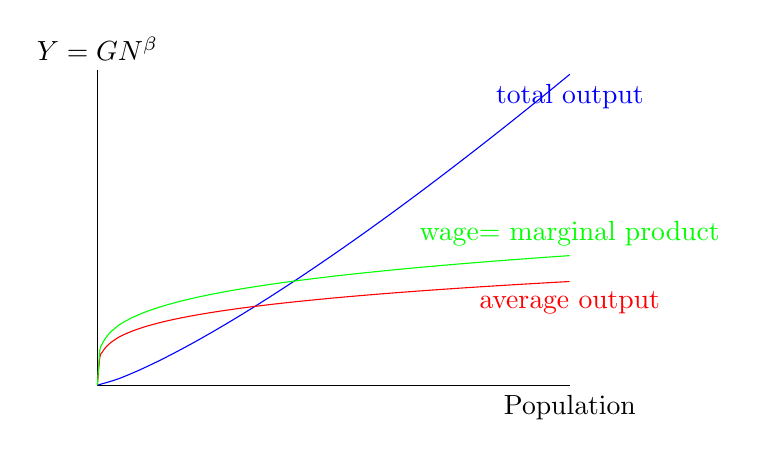
\begin{tikzpicture}
      \draw (0,4)node[above]{$Y= GN^{\beta}$}--(0,0) --(6,0)node[below]{Population};
       \draw[scale=1, domain=0:6, smooth, variable=\x, blue] plot ({\x}, {(\x/2)^1.25})node[below]{total output };% divide by 2 to get it on the plot
       %\draw (0,1)node[left]{$\alpha$}--(6,3.5)node[left]{$\alpha +\rho P$};
      \draw[scale=1, samples=200,domain=0:6, smooth, variable=\x, red] plot ({\x}, {(\x/2)^.25})node[below]{average output};% THis is the wage plot
    \draw[scale=1, samples=200,domain=0:6, smooth, variable=\x, green] plot ({\x}, {(1.25*(\x/2)^.25)})node[above]{wage= marginal product};
%[red] plot[samples=200, domain=-0:6] function {(\x/2)^.25}node[above]{wage};
      %  \node [left] at (0,2){$w=\rho P$};
         % \draw [dashed](0,3)node[left]{$Y_i$}--(6,3);
    \end{tikzpicture}\vspace{.5cm}
    \caption{Urban productivity is proportional to population, $\beta=1.13$}
    \label{fig-scale-output}
    \end{center}
\end{figure}

The right hand side of second equation is derived from the first bvy differentiation and combined with a result from the theory of the firm that says that the firm should hire until the marginal value product of labour is equal to the total wage, $\omega+w$, where $w$ is the `subsistance wage' that is earned by non-urban workers.  
\[\omega+w = \beta GN^{\beta-1}\]

The third is the population equilibrium condition, that requires that at the boundary of the city, $d^*$,  transportation costs, $td^*$, consume the entire wage:
 \[d^*=\frac{\omega}{t}\]

 The fourth is the function that generates the total urban poulation. In the standard circular city, for example, with a uniform density, $\delta$,  
 \[N=\delta\pi (d^*)^2\]
 % \[N=\delta\pi (\frac{\omega}{t})^2\]
 %\[N=\delta\pi (\frac{\beta GN^{\beta-1}-w}{t})^2\]
 
 The equilibrium population  is: 
% \[N=\delta\pi (\frac{\beta GN^{\beta-1}-w}{t})^2\]

\begin{eqnarray}
    N&=&\delta\pi (\frac{\beta GN^{\beta-1}-w}{t})^2\\
    &=&\frac{\delta\pi }{t^2} \left[\beta GN^{2\beta-2} -w^2\right]
\end{eqnarray}

This expression can be treated as a difference equation if we consider the left hand side as $M_{c}$ and the right hand side  function of the previous period's as population, $N_{{c}-1}$.



\subsection{Incorporating Agglomeration Economies in Production} \label{sec-agglomeration-production}
%Production economies generated by agglomeration enter the production functions of the firms and, indirectly,  the aggregate production function of the city. 
A simple way  to introduce an agglomeration effect on the production side that is consistent with the existing literature is  to use a \gls{Solow-Swan model} with labour augmenting technical change (\cite{solowContributionTheoryEconomic1956, swanEconomicGrowthCapital1956}), $Y(t)=K(t)^{\alpha }(A(t)n)^{\beta }$ where $t$ denotes time,  %$0<\alpha<1$ is the elasticity of output with respect to capital, $\beta$ the elasticity of output with respect to effective labour,
 and $Y (t )$  represents total production. 
We %remove time  $t$ except in the technical change term, where we replace it with the population value $n$. To avoid confusion with the consumption amenity, we
 replace $A(t)$ %in the Solow-Swan models
  with $A(n)$, representing a labour-augmenting agglomeration effect.\footnote{The Mankiw–Romer–Weil version of the model adds a term for human capital.  It is not clear it would make a qualitative difference for our analysis.}  This differs from  the Slow-Swan, model in which labour augmenting technical change increases according to an exogenous (exponential) law.\footnote{An attractive ways to specify $A(n)$  is to use a simple exponential, $A(n)=n^\phi$, which changes Equation~\ref{eqn-solow-swan2} 
  We %The model  can produce increasing returns in the aggregate, which can drive city growth.
\begin{eqnarray}
 Y&=K^{\alpha }(n^{\phi }n)^{\beta}  \nonumber\\
 Y&=K^{\alpha }n^{\beta(1 +\phi)}
\label{eqn-solow-swan1}
\end{eqnarray}
This makes it clear that we can have increasing returns to scale for the urban economy if  $\alpha + \beta(1+ \phi)>1$ even with a production function at the firm level that is decreasing returns to scale ($\alpha +\beta<1$)).\label{footnote-psi}}  
%Rising transportation costs may become the limit on firm or city expansion.  
  
  $A(n)n$ is  ``effective labour'' and 
%\footnote{The Mankiw–Romer–Weil version of model adds a term for human capital.  It is not clear it would make a qualitative difference for our analysis.}  $T$ refers to effect of \textbf{labour-augmenting agglomeration}. The model then says that the 
firm output is 
\begin{equation} 
Y=K_i^{\alpha }(A(n)n_i)^{\beta }
\label{eqn-solow-swan2}
\end{equation}
% If $\beta=1-\alpha$, this is a constant returns to scale (CRS) production function. Without agglomeration effects, $T(n)=1$,  Then 
% \textbf{$\mathbf{L(n) = T(n) n}$ 
An individual firm will purchase labour time  and sell the product of effective labour. 
?If labour markets are competitive, it will set $\die{Y}{L}=w$.
We can assume  that $A(1)=1$ and $\frac{\partial A}{\partial n}>0$. 

Notice that this model ascribes all agglomeration effects to labour rather than capital Deepening  and widening of the labour pool was one of Marshall's explanations of the formation of industrial districts. The model can therefor  be seen as incorporating a Jacobs/Marshall externality (\cite{beaudryWhoRightMarshall2009, vanderpanneAgglomerationExternalitiesMarshall2004}) of the sort often invoked as an explanation of industrial clusters. These externalities  are not a product of any firm or individual. 



\subsection{Labour demand}\label{sec-labour-demand}
%This equation shows labour supply increasing with the square of the wage.  
%The  inverse labour supply function  is
%	\begin{equation}
%	w= (\frac{ {c}^2s}{\pi})^{0.5} L^{0.5},	%\label{eqn-inverse-labour-supply}
%	\end{equation}
%which is clearly increasing with the square root of the wage. 
%It's easier to show the wage curve is declining at a faster rate withthis equation. 

%K The marginal product of labour is declining. While adding more labour may always adds some value, the rate drops off.  If the marginal product increased, then a firm that got large enough would out compete smaller firms, hire all labour, always be able to produce more wealth by hiring more people, and would always produce more wealth by hiring people than by firing people. This doesn't happen.

%K Perhaps, the firm hires employees who best fit its needs first, but to grow, eventually it must hire less selectively. Finding markets may get harder with growth. Perhaps expansion adds additional costs, building a parking lot, administration, acquiring    a larger building. Whatever the explanation, the marginal product of labour declines. 

Profit maximizing firms  set the marginal value product of labour, $p\frac{\partial Y_i}{\partial n_i}$, equal to the wage. The marginal product of labour, however,  is complicated by the presence of the  agglomeration effect, $A(\sum n_j)$:
\begin{eqnarray} \frac{\partial Y_i}{\partial n_i} &=   K_i^\alpha \left(  \beta A n_i^{\beta-1}  + n_i^{\beta}A'  \right)  \nonumber\\
&=   \beta\frac{1}{n_i} Y_i   +  Y_i \frac{A'}{A}  \nonumber\\
&=   Y_i  \left[  \beta\frac{1}{n_i}  + \frac{A' }{A} \right]   \label{eqn-mpl}
\end{eqnarray}
The first term in the square bracket in Equation~\ref{eqn-mpl} might be termed the \textbf{private myopic marginal product}. It is the addition to output directly attributable to an additional worker. This myopic MPL is smaller than the actual marginal product for the firm.  
The second term in the bracket   is the marginal agglomeration effect. It captures the effect on firm-wide labour productivity -- an increase in effective labour --   that results from adding a worker. We can expect this to be very small.\footnote{Using the specification in Footnote~\ref{footnote-psi}, $Lambda(n)=n^\psi$, it would be $\frac{\psi}{n}$. If f $\psi=0.1$ and $n=250,000$ the number is $\frac{A' }{A} =4\times 10^{-7}$.}% REVIEW THIS 
% REVIEW THIS TOO
%\footnote{Firm size matters. 
%A monopoly employer would take into account the marginal agglomeration effect. 
%A firm that employed a large enough fraction of the urban workforce to notice agglomeration effects, say $\frac{1}{n}<k<1$, would enjoy that fraction of the external effect and set the wage at  
%\[w_k =  \beta\left( \frac{1}{n}+ \frac{kA'}{A(n)} \right)	Y\].} 


It seems likely that the agglomeration effect of adding a worker on the productivity of other workers in that firm, $Y_i \frac{A'}{A}$, would be difficult to attribute to a new worker. It would be a lagged, unevenly distributed effect, and would appear exogenous, and so would not be compensated. We assume therefore that firms do not take the second term into account. %If we also assume that firms take the wage as parametric, firms hire until the private myopic marginal product falls to the observed wage, 
%		\[  \beta\frac{1}{n_i} Y_i =    w+\phi , \]
implying firms will hire fewer than the optimal number of workers.
\begin{table}[htbp]
\caption{Four views of the of the marginal agglomeration effect, $\frac{A'}{A}$}
\begin{center}
\begin{tabular}{rlcccc}\small
    & 	\hspace{2cm}$\frac{A'}{A}=$	& $.01$ & $.01$ & $.001$  &  $4\times 10^{-7}$\\ \cline{3-4}
\   &  	version  		& 1 firm 		&10 firms		&100 firms 	& 1000 firms		\\ \hline%\cline{3-5}
 1 &myopic 		&0 			& 0			& 0       		&	0				\\
 2 &firm wide, 0CV 	& $0.01Y$		& $0.01Y_i$	& $0.001Y_i$	& $4\times 10^{-7}Y_i$	\\
 3 &firm wide, 1CV	& $0.01Y$		& $0.1Y_i	$	& $0.1Y_i$	&$4\times 10^{-4}Y_i$	\\
4  &social 			& $0.01Y$ 	&  $0.1Y$		& $10Y_i$		&$4\times 10^{-4}Y_i$	\\
 \hline
\end{tabular}
\end{center}
\label{table-marginal-agglomeration}
\end{table}%


Even taking into account firm-wide labour productivity gains, the private marginal product of labour is likely to be computed on the assumption that other firms do not expand  their workforce. This could be call the `zero conjectural variation' (0CV) case. If all firms  were expected to respond to the same signal the same way (1CV), the agglomeration effect  would be multiplied by the number of firms, $\frac{n }{n_i}$. The marginal agglomeration effect for firm $i$ is then $\frac{n }{n_i}\frac{A' }{A}Y_i =\frac{A' }{A}Y$. 

Since the increase in $A$ affects all firms, the  social marginal product of all firms expanding their workforce by one worker as $i$ does must be multiplied again by the number of firms. The  value of the agglomeration effect increases with the number of firms. 

\begin{figure}[tb]
\begin{center}

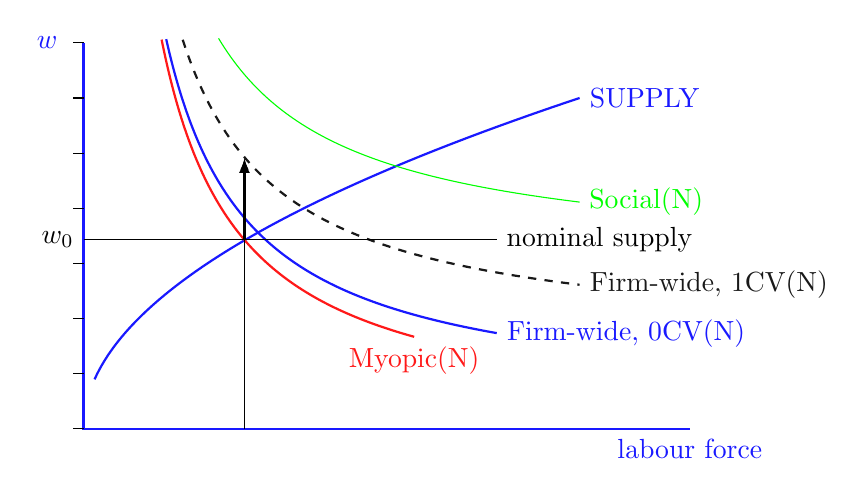
\begin{tikzpicture}[scale=.7]
%\def\bndmax{5}        %https://tex.stackexchange.com/questions/68462/filling-a-complex-region-with-tikz
%\def\bndmin{0.2}
\def \Y {7}  % height of y axis pecent
\def \W {15}  % length  of x axis
\def \Wbar {3} % jmeam wealth
\def \omega {3}
\def \A {1}  %was .5
\def \B {.5}

\draw [thick, color=blue!90] (0,\Y)node[left=.2cm]{$w$} -- (0,0)--(\W-4,0)node[below]{labour force};  
 \foreach \yi in {0,...,\Y} \draw (0,\yi)--(-.2,\yi)node[left]{};
 
\tikzset{func/.style={thick,  color=blue!90}}
\draw[ func, domain=.2:\W-6] plot [samples=200] (\x, 2*\x^.5)node[below=.1, right]{SUPPLY};

\tikzset{func/.style={  color=green}}	
\draw[func, domain=2.45:\W-6] plot [samples=200] (\x, 10/\x+3)node[above=.1, right]{Social(N)};

\tikzset{func/.style={thick, dashed, color=black!90}}	
\draw[func,domain=1.8:\W-6] plot [samples=200] (\x, 10/\x+1.5)node[ right]{Firm-wide, 1CV(N)};

\tikzset{func/.style={thick, color=blue!90}}	
\draw[func,domain=1.5:\W-7.5] plot [samples=200] (\x, 10/\x+.4)node[below=.05, right]{Firm-wide, 0CV(N)};

\tikzset{func/.style={thick,color=red!90}}	
\draw[func,domain=8.5/6:\W-9] plot [samples=200] (\x, 10/\x)node[below]{Myopic(N)};

\draw(0,3.425)node[left]{$w_0$}--(7.5,3.425)node[right]{nominal supply };
\draw[thin,-latex](2.92,0)--(2.92,4.9); %a vertical labour supply
\draw[thick,-latex](2.92,3.425)--(2.92,4.9);
%\draw [blue,  thick](13, 8.3)--(15,8.3)node [right, black] {\small A=\ 1,\ B=0.5};
%\draw [green, thick](13, 7.6)--(15,7.6)node [right, black] {\small A=.8, B=0.8};

%\node at (5,-1.5){Resulting in  profits, expansion, and/or entry: the city grows};
 \end{tikzpicture}
\caption{Multiple Marginal Products - check}
\label{fig-growth-amenity.tex}
\end{center}
\end{figure}

 illustrates the labour supply curve and the four versions of MPL that arise for any standard production function with diminishing marginal product of labour and agglomeration effects of the sort we model. These agglomeration effects account for O'Sullivans axioms (b), (c) and (d) for this and similar models. 

 
\subsubsection{Output and wage}
We need a combination of classical and neoclassical distribution theory.

City output is divided among the classes of society. Neoclassical theory suggests wages are allocated according to marginal product and classical theory suggests rents according to the pattern of ownership.

Equation one, in effect determines a wage, (Given the observed values for the scaling coefficients for total wages and labour, $bW < 1.15$ and $bL < 1$, )  although there are many possible distributional specifications and many possible labour market and firm structures. Bettencourt provides two  estimates,  1.11 and 1.35, for the scale factor for urban personal income in the Brazil and South Africa respectively. A more recent  study supports the Bettancourt results for China.\footnote{Wu W, Zhao H, Tan Q, Gao P. An Urban Scaling Estimation Method in a Heterogeneity Variance Perspective. Entropy (Basel). 2019 Mar 28;21(4):337. doi: 10.3390/e21040337. PMID: 33267051; PMCID: PMC7514821.} 

\subsubsection{Wage and city size}
The third determines the extent of the city. This comes form the Alonzo model discussed in chapter XXXXA. 

% PROBABLY REMOVE - FIGURE REPEATS
\begin{figure}
    \begin{center}
     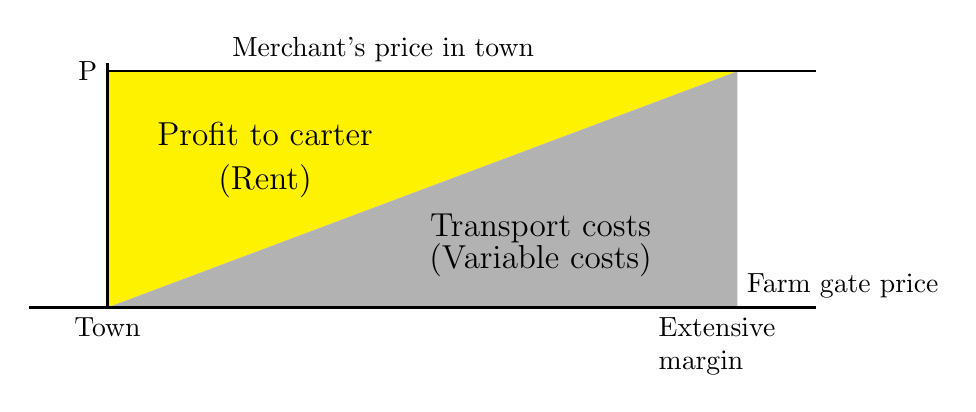
\begin{tikzpicture}[domain=0:2]
%\draw[thick,color=gray,step=.5cm, dashed] (-0.5,-.5) grid (3,3);
%\draw[line width=.01, green ] (0,0) -- (10,0) node[right  ] {Distance};
\node at (1,0) [below] {Town};
\fill[yellow]  (1,0) --(9,3)--(1,3) --cycle;
\fill[gray!60] (9,3) --(1,0)--(9,0) --cycle;

\draw[thick ] (1,3)node[left]{P}  -- (10,3);\node at (4.5,3)[above ] {Merchant's price in town} ;
\draw[thick ] (0,0)  -- (10,0); 

%\draw[thick,color=red] (1.5,0) -- (1.5,1) node[below right] {Fixed cost} -- (1.5,1.5) --(10,3.25)node[above left] {total cost};
\draw[thick] (1,0) -- (1,3.1) ;
\node[below,text width=2cm]at (9,0) {Extensive margin};
%\draw[ultra thick, blue,<-> ] (3,1.8) -- (3,2.5)node[left] {annual rent at a} -- (3,3) ; 
\node at (9,0)[above right] {Farm gate price};
\node  at (6.5,1){\large Transport costs};
\node  at (6.5,.6){\large (Variable costs)};
\node  at (3.,2.2){\large Profit to carter};
\node  at (3.,1.6){\large (Rent)};
\end{tikzpicture} 
    \caption{Transport costs, the yellow area, take a share of the profit for vegetables sold in the town}
    % \label{fig-rent-ricardo}
    \end{center}
\end{figure}

\begin{figure}
    \begin{center}
    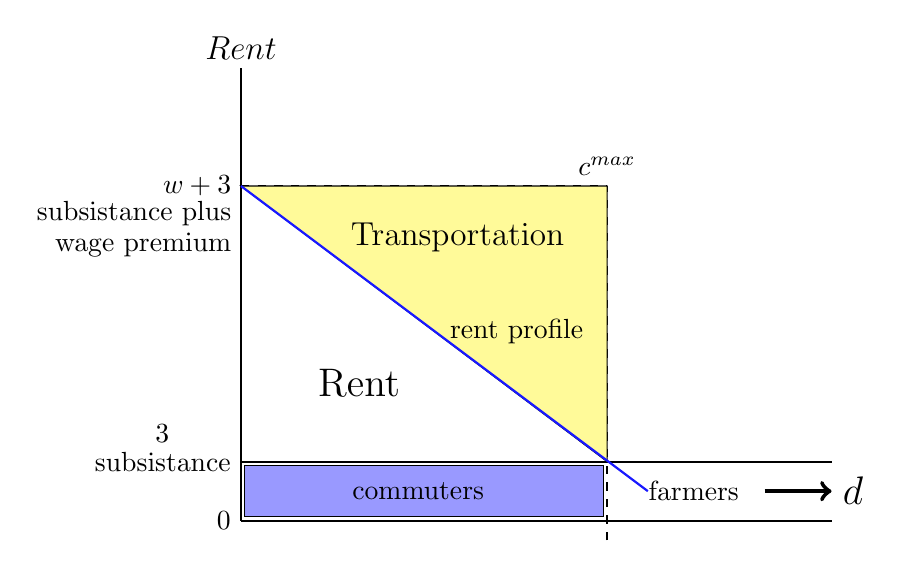
\begin{tikzpicture}[scale=.5]
\def\bndmax{5}        
\def\bndmin{0.2}
\def \n {10}  % height of y axis
\def \d {15}  % length  of x axis
\def \t {.75}  %  cost of transportation per unit x
\def \th {1}   %
\def \w {7}    %  wage premium
\def \om{1.5}%  omega =rural wage Zero for urban population
\def \azero{2}
\def \aprime {-.0}	
\tikzset{func/.style={thick,color=blue!90}}	
\draw [thick] (0,-\om) --(\d,-\om);  			% Zero for rural population
\draw [thick] (0,-\om)node[left]{$0$} --(0,\n);	% Y axis
\node at (0,\n+0.5){\large$Rent$};

\draw [thick] (0,0)node[left]{subsistance}--(\d,0);
\node a t(-2,.7) {$\omega$};
\node[left] at (0,\w){$w+\omega$};
\node[left] at (0,\w-.7){subsistance plus};
\node[left] at (0,\w-1.5){wage premium};	
\draw [dashed, thick](9.3,-2)-- (9.3,\w)node[above]{$c^{max}$};
\draw [dashed, thick](0,\w)-- (9.3,\w);
% solid color for commuters
\draw[fill=blue!40] (0.1,-0.1) rectangle (9.2,-\om+.1);
\draw[fill=yellow!40] (9.30,7.) -- (0,7)--(9.30,0.)--cycle;% Rent \w-.2
\draw[func,domain=0:\w/\t+1] plot [samples=200] (\x,{\w-\t*\x});
\node at (5.5,5.7){\large Transportation};
\node at (7,3.3){rent profile};		%Rent Profile	
\node at (3.,2){\Large Rent}; 		%Rent 
\node at (4.5,-\om/2){commuters};
\node at (11.5,-\om/2){farmers};
\draw [ ultra thick, ->](13.3,-\om/2)--(15, -\om/2)node [right] {\Large $d$};
\end{tikzpicture}
    \caption{A circular city with uniform transportation costs.}
    \label{fig-rent-alonzo}
    \end{center}
\end{figure}

A simple case is the circular city with uniform transportation cost, $t$. \[r^*= \frac{w}{t}\]% A more complex model might have density depend on location, for example, in the continous circular cityt\,
If transportation costs vary by  distance we might have something like this constraint on extent\[w=\int_0^{d*} t(d)dt.\]

This approach imposes an equilibrium condition on the model. It is unnecessary working with a citation of known extent and density. The analytic approach is easily extended to variable transportation cost, although at the expense of additional computational complexity.

\subsubsection{City extent and population}
Equation  four  closes the model by linking the extent of the city to the population. A simple case is the circular city with uniform population $d$, where $d$ is density per unit area and $r^*$ is the radius of the city: \[P=d\pi r^{*2}\] 
More generally, density might vary with for example, the distance $r$ from the centre of the city:
\[P=\pi \int_{0}^{r*}d(r)\,dr\] 
In a computational model a table of densities would provide the link.



\subsubsection{challenges}
maybe discuss some of the modeling challenges - division of income, lags, ???

\vspace{2cm}

 The growth of many cities was initially fueled by agricultural rents and resource exports. The industrial revolutions transformed many of these consumption cities into thriving production centers. 

while the ``origins'' of consumption cities can be traced to (i)
resource rents, (ii) rents from agricultural exports in countries with sufficiently high agricultural productivity, and (iii) ``premature'' deindustrialization.  Source:
%\href{https://www.brookings.edu/blog/future-development/2022/07/14/1622441/}
{Are cities engines of production or consumption, and does it matter?}




\subsection{Rent seeking}
  Rent-seeking is the act of growing one's existing wealth without creating new wealth by manipulating the social or political environment. Rent-seeking activities have negative effects on the rest of society. They result in reduced economic efficiency through misallocation of resources, reduced wealth creation, lost government revenue, heightened income inequality,


\section{MOVE: agglomeration factors and returns to scale}

So we have a a population, $n$, and a wage, determined endogenously by competitive markets. 
EXPLAIN - AND WHERE DOE STHIS GO?
If labour markets are \gls{competitive market}, we set die${Y}{L}=w$ .

---

MOVE ro
To maximize profit  firms set the marginal value product of labour, $p\die{Y_i}{n_i}$, 
equal to the wage. 

MARGINAL VALUE VS MARGINAL PRODUCT
in a competitive market, firms offer a wage equal to marginal value of labour, 
 $p\die{Y_i}{n_i}$, where $i$ indicates the $i^{th}$ firm. In the analytic model, there is no \gls{frictional unemployment}, there are no \glspl{labour adjustment cost}. 

 For convenience, price per unit is one. 

A labour market equilibrium exists if the marginal product of labour, is monotonically declining, which it is with a \gls{Cobb-Douglas} production function, and $\alpha + \beta<1$ 
Population would be expected to adjust much more slowly than firm wages, so labour supply should converge.

The marginal product of labour declines monotonically, to ensure there is a labour market equilibrium, in order to maintain a strong link to the analytical modelling tradition.
% ***ILLUSTRATE AND CLARIFY
% If you see it as just supply and demand .. 
% Supply demand with fixed product and everything’s neat
% Agglomeration changes everything. firms are underestimating each time they add a worker, the value that’s going to be produced. They benefit from an agglomeration effect and that’s where they interesting dynamics are coming from..
% we know that there is a marginal product of labour for a firm that it should be able to figure it out.. can the person on the shop floor figure out whether it's worth hiring another person.. we can talk about it, add details etc. We have a declining marginal product of labour. Because of transportation costs, we have a rising cost of getting labour so they cross and there is an equilibrium. There are adjustment questions like which adjusts quickly, how fast people move in, how fast firms decide to hire etc, but we know that there is in principle and equilibrium and that it is in principle a stable equilibrium (DIAGRAM STROGATS) although there are complications with this-- some argue these market equilibria never make sense- true in lots of way, but useful for analysis. 
% The question is then, what happens in our city? Do you get a growth dynamic? What seems to be the case is that if all the firms add workers then the marginal value of the product of all the workers they have goes up, which means they are making more profit which means if they are making more profit they want to hire more workers? Does it ever converge? Likely eventually, but it's got a very powerful dynamic.  If you add other features like more products being created in the city, which is part of this agglomeration process you can start seeing, if you exhaust one source of growth, we know that there are others, that simplification is just firms of the same sort hiring workers of the same sort is wrong. so we need to add the local service sector, we need to add the possibility of creating new products and those depends on the number of workers and so depend on further agglomeration effects. What does this mean? For the purpose of the model, we'd want to strengthen the agglomeration effect relative to what they are for specific firms or industries..



MOVE?

 Notice that this formulation implies it is possible to have increasing returns to scale for the urban economy even with a production function at the firm level with decreasing returns to scale: the return to the total economy $\alpha + \beta(1 + \gamma)$ can be greater than one, even if $\alpha +\beta$ is less than one. %.\label{Fn:PSI}}  (CITE Appendix: Excess Returns)
 
The \gls{agglomeration effect} means that although individual firm returns to scale are declining, the city can experience \gls{increasing returns to scale} in the utilization of human capital. % NEED? Individual firms have decreasing returns, but the presence of agglomeration economies external to firms but internal to the city gives the urban economy as a whole increasing returns to scale .}.
%\footnote{The formulation is consistent with the discussion of endogenous growth theory in Chapter \ref{chapter-growth}, which demonstrated that increasing returns at the macro level is consistent with decreasing returns at the micro level. The effects are not limited to the individual firm. \Gls{spillover effects} can be large, see section \ref{section-spillover}. }





